\noindent\textcolor{red}{\textbf{R\#2}}\,\textcolor{blue}{\textbf{W1:}}We thank the reviewer for raising this important concern and clarify why the anticipated FAR degradation does not occur. \textbf{(i)} CU maps each forget class to its nearest retain \emph{centroid} (Eqs.~2 and~3), and to suppress the forget response we employ a ReLU margin $\gamma$ (Eq.~5) between the forget and retain logits. This margin enforces a sufficient angular gap, so a forget probe does not match a retain identity under cosine similarity, even with a single sample per identity (table below). CU gives FAR@0.5\,$=$\,\textbf{3.83\%} and EER\,$=$\,\textbf{24.99\%}, on par with the Oracle (\textbf{3.10\%}, \textbf{21.69\%}), and both rise similarly over \emph{Before} (1.64\%), so this small rise comes from removing the identities, not confusing them. A forget probe matches a retain identity only as often as a random stranger, and the forgotten identity is genuinely destroyed, recoverable only by retraining. It is therefore confounded with no one, so the design is \textbf{not ill-posed} and CU does not reduce security. \textcolor{red}{\textbf{R\#2}}\,\textcolor{blue}{\textbf{W2}}, \textcolor{red}{\textbf{R\#3}}\,\textcolor{blue}{\textbf{W4:}} We thank the reviewer for these points. We add standard verification metrics in Table~\ref{tab:more_results} (FAR at $0.3,0.4,0.5$ and EER), which are embedding-distance (open-set) scores rather than class attribution, with the same trend across all four modalities. The replay set $D_r$ ($10\%$ of $D_r^{full}$) is used only during unlearning and contains at least one sample per retain identity ($\approx 42$ classification, $\approx 32$ face, $1$ to $2$ iris, $1$ fingerprint); all retain numbers are reported on the full held-out test split of $D_r^{full}$, not on $D_r$. As discussed in Sec.~6.1, a minimal $D_r$ is unavoidable for non-convex deep models, while feature-level, source-free, and synthetic replay alternatives are limited to convex or generative settings. $D_r$ holds only consenting retain identities; a withdrawal is handled as a forget request and the buffer is refilled from the remaining consenting pool, consistent with limited lawful processing under GDPR and CCPA. \textcolor{red}{\textbf{R\#2}}\,\textcolor{blue}{\textbf{W3:}} We thank the reviewer for this helpful suggestion. Following the criterion in our paper Sec.~6 and Fig.~6, a well-learned model concentrates attention on facial regions such as the forehead, nose, and chin, whereas an unlearned model or one never exposed to an identity spreads attention to hair, background, and corners. For forget samples the base model focuses on the face while the retrained and CU models shift to the background, confirming identity removal. We add the retain case in Fig.~\ref{fig:updated_atten}. For retain samples the base, retrained, and CU models all keep attention on facial regions, confirming retain identities are preserved. This shows CU is surgical, pushing attention to the background for forget identities while keeping it on facial cues for retain identities, as described in the paper. \textcolor{red}{\textbf{R\#2}}\,\textcolor{blue}{\textbf{W4:}} We thank the reviewer and clarify both metrics. MIA follows the label-only attack of \cite{choquette2021label}, combining gap, boundary-distance, and augmentation attacks. We report attack accuracy on member (forget-train) versus non-member data, where $0.5$ means the attacker cannot infer membership and thus successful forgetting. KL divergence is reported separately as $\mathrm{KL}(\mathcal{M}_{\text{unlearned}} \,\|\, \mathcal{M}_{\text{oracle}})$ over the evaluation set, measuring how close the unlearned model is to the oracle. \textcolor{red}{\textbf{R\#2}}\,\textcolor{blue}{\textbf{W5,W6}}, \textcolor{red}{\textbf{R\#3}}\,\textcolor{blue}{\textbf{W1:}} Algorithm~\ref{alg:cu} is the corrected, consistent version. \textcolor{red}{\textbf{R\#2}}\,\textcolor{blue}{\textbf{W7}}, \textcolor{red}{\textbf{R\#3}}\,\textcolor{blue}{\textbf{W2:}} We thank the reviewer. The local loss is now included in Algorithm~\ref{alg:cu}. $\mathcal{L}_{\textit{local}} = \lambda_{\textit{local}} \sum_{g=1}^{G} \|\theta_g\|_2$ is a group-Lasso with one group per block, where $\theta_g$ start at zero, so it penalizes the change from the pretrained model rather than the absolute magnitude. The group $\ell_2$ norm drives entire blocks to zero update, so larger changes are penalized more and only a few blocks change, giving the surgical updates.
\begin{center}
\footnotesize\setlength{\tabcolsep}{4pt}
  \begin{tabular}{lcccc}\hline
  \textbf{Model} & \textbf{FAR@0.3} & \textbf{FAR@0.4} & \textbf{FAR@0.5} & \textbf{EER}\\\hline
  Before & 11.38\% & 4.84\% & 1.64\% & 13.33\%\\
  CU & 17.97\% & 8.52\% & 3.83\% & 21.99\%\\
  Oracle & 16.10\% & 7.79\% & 3.10\% & 21.69\%\\\hline
  \end{tabular}
  \captionof{table}{FAR/EER of $D_f$ probes against $D_r$ on CASIA-Iris.}
  \label{tab:more_results}
  \end{center}

\begin{figure}[!ht]
    \centering
    \vspace{-6pt}
    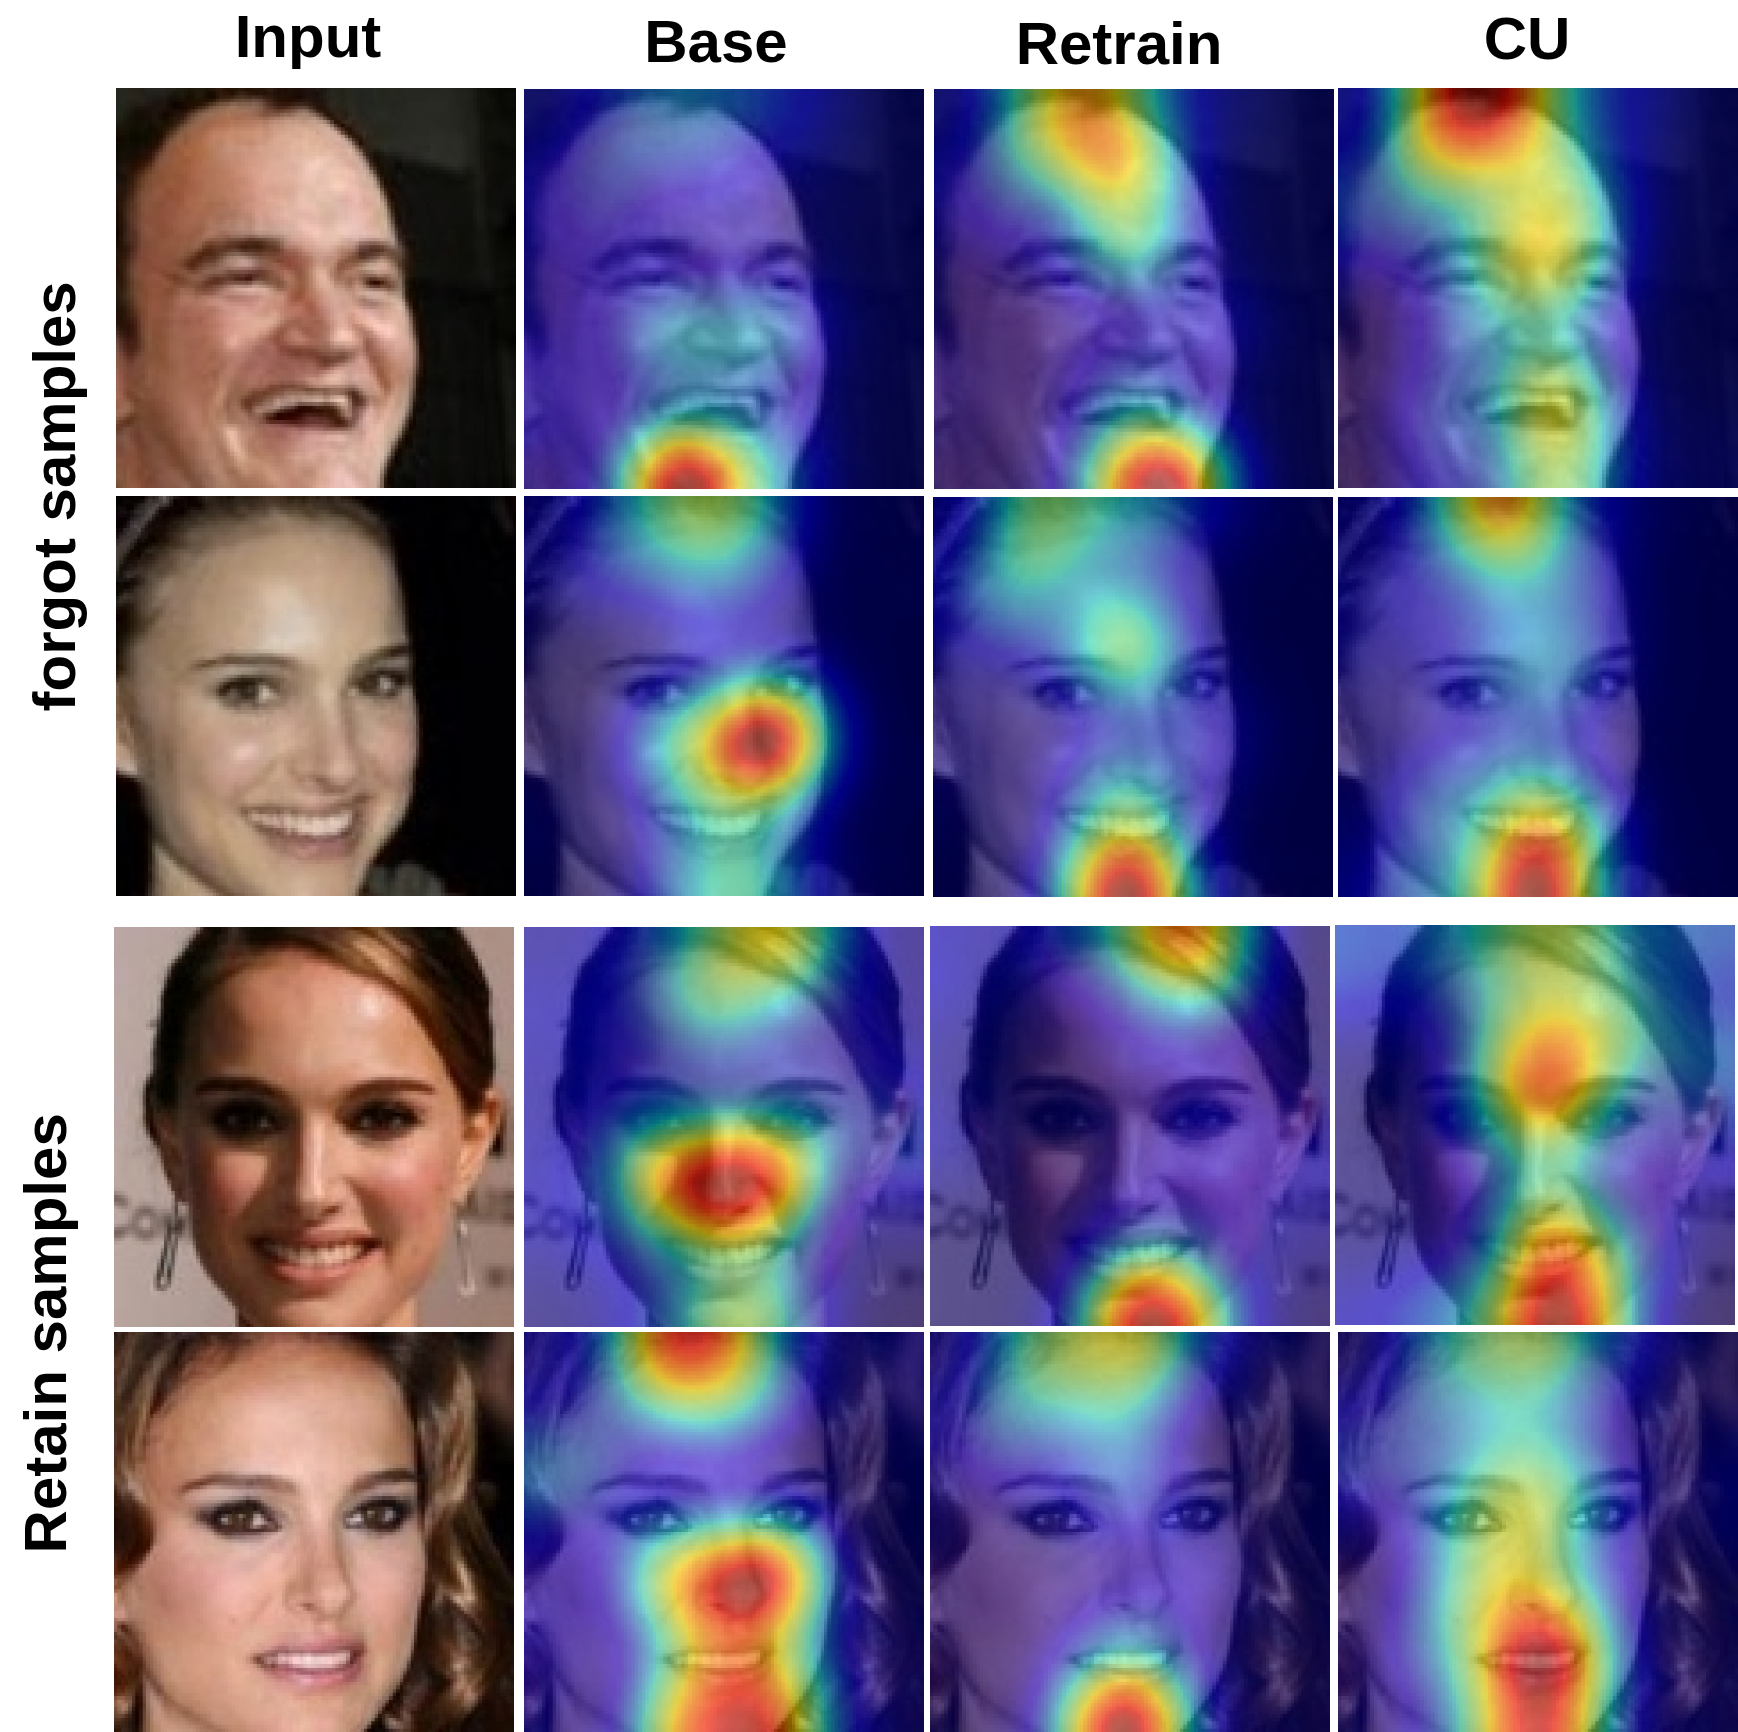
\includegraphics[width=0.5\linewidth]{images/atten.png}
    \vspace{-4pt}
    \caption{Attention maps on forget and retain samples.}
    \label{fig:updated_atten}
\end{figure}

\begin{algorithm}[htbp]
\caption{Camouflage Unlearning}\label{alg:cu}
\begin{algorithmic}[1]
\scriptsize
\newcommand{\eb}[1]{\operatorname{emb}(#1)}
\newcommand{\Ld}{\mathcal{L}_{\text{dom}}}
\newcommand{\Lr}{\mathcal{L}_{\text{ret}}}
\newcommand{\Ll}{\mathcal{L}_{\text{local}}}
\newcommand{\Lt}{\mathcal{L}_{\text{total}}}
\newcommand{\Lf}{\mathcal{L}_{f}}
\Require $\mathcal{M},D_f,D_r,\gamma,\lambda_{\text{dom}},\lambda_{\text{ce}},\lambda_{\text{emb}},\lambda_{\text{local}},E$
\Ensure Unlearned $\mathcal{M}'$
\For{each class $k\in D_r\!\cup\!D_f$}
    \State $c_k\!\gets\!\tfrac{1}{|D_k|}\sum_{x\in D_k}\eb{x}$ \hfill\Comment{Eq.~1}
\EndFor
\For{each forget class $i$}
    \State $j^*\!\gets\!\arg\min_j\|c_{f_i}\!-\!c_{r_j}\|_2$;\;$\mathbf{t}_i\!\gets\!c_{r_{j^*}}$ \hfill\Comment{Eq.~2,3}
\EndFor
\For{$e=1$ \text{to} $E$}
    \For{each mini-batch $(D_f,D_r)$}
        \State $\Lf\!\gets\!\tfrac{1}{|D_f|}\sum_{\mathbf{x}\in D_f}\|\eb{\mathbf{x}}\!-\!\mathbf{t}_y\|^2$ \hfill\Comment{Eq.~4}
        \State $\Ld\!\gets\!\operatorname{ReLU}(\max_{i\in F}z_i\!+\!\gamma\!-\!\max_{j\in R}z_j)$ \hfill\Comment{Eq.~5}
        \State $\Lr\!\gets\!\lambda_{\text{ce}}\operatorname{CE}(\mathbf{z}_r,y_r)+\lambda_{\text{emb}}\tfrac{1}{|D_r|}\sum_{\mathbf{x}\in D_r}\|\eb{\mathbf{x}}\!-\!c_y\|^2$ \hfill\Comment{Eq.~6}
        \State $\Ll\!\gets\!\lambda_{\text{local}}\sum_{g}\|\theta_g\!\|_2$ \hfill\Comment{Eq.~7}
        \State $\Lt\!\gets\!\Lf\!+\!\lambda_{\text{dom}}\Ld\!+\!\Lr\!+\!\Ll$ \hfill\Comment{Eq.~8}
        \State Update $\mathcal{M}$ via $\nabla_\theta\Lt$
    \EndFor
\EndFor
\State \Return $\mathcal{M}'$
\end{algorithmic}
\end{algorithm}
